%===================================================================
\section{Experimental Results}
%===================================================================

\subsection{Training Run Summary}
All results are from the \texttt{rl\_last} training run using the Wave Bonus reward scheme at Difficulty 1. Model checkpoints were saved at every episode.

\begin{table}[htbp]
\centering
\caption{Training Performance Summary (193 Episodes, $\sim$262k Steps)}
\label{tab:results}
\begin{tabular}{@{}lc@{}}
\toprule
\textbf{Metric} & \textbf{Value} \\
\midrule
Total episodes & 193 \\
Total environment steps & 262,913 \\
Average episode length (ep 1--10) & 1,298.5 steps \\
Average episode length (ep 184--193) & 1,433.6 steps \\
Survival Length improvement & \textbf{+10.4\%} \\
Avg kills (ep 1--10) & 5.6 \\
Avg kills (ep 184--193) & 8.1 \\
Kill improvement & \textbf{+44.6\%} \\
Peak episode reward & 6,278.6 (ep 185) \\
Peak kills (single episode) & 27 (ep 185) \\
Peak survival length & 2,191 steps (ep 28) \\
Q-loss (ep 1 $\to$ ep 193) & 2.80 $\to$ 3.38 \\
\bottomrule
\end{tabular}
\end{table}

\begin{figure}[htbp]
\centering
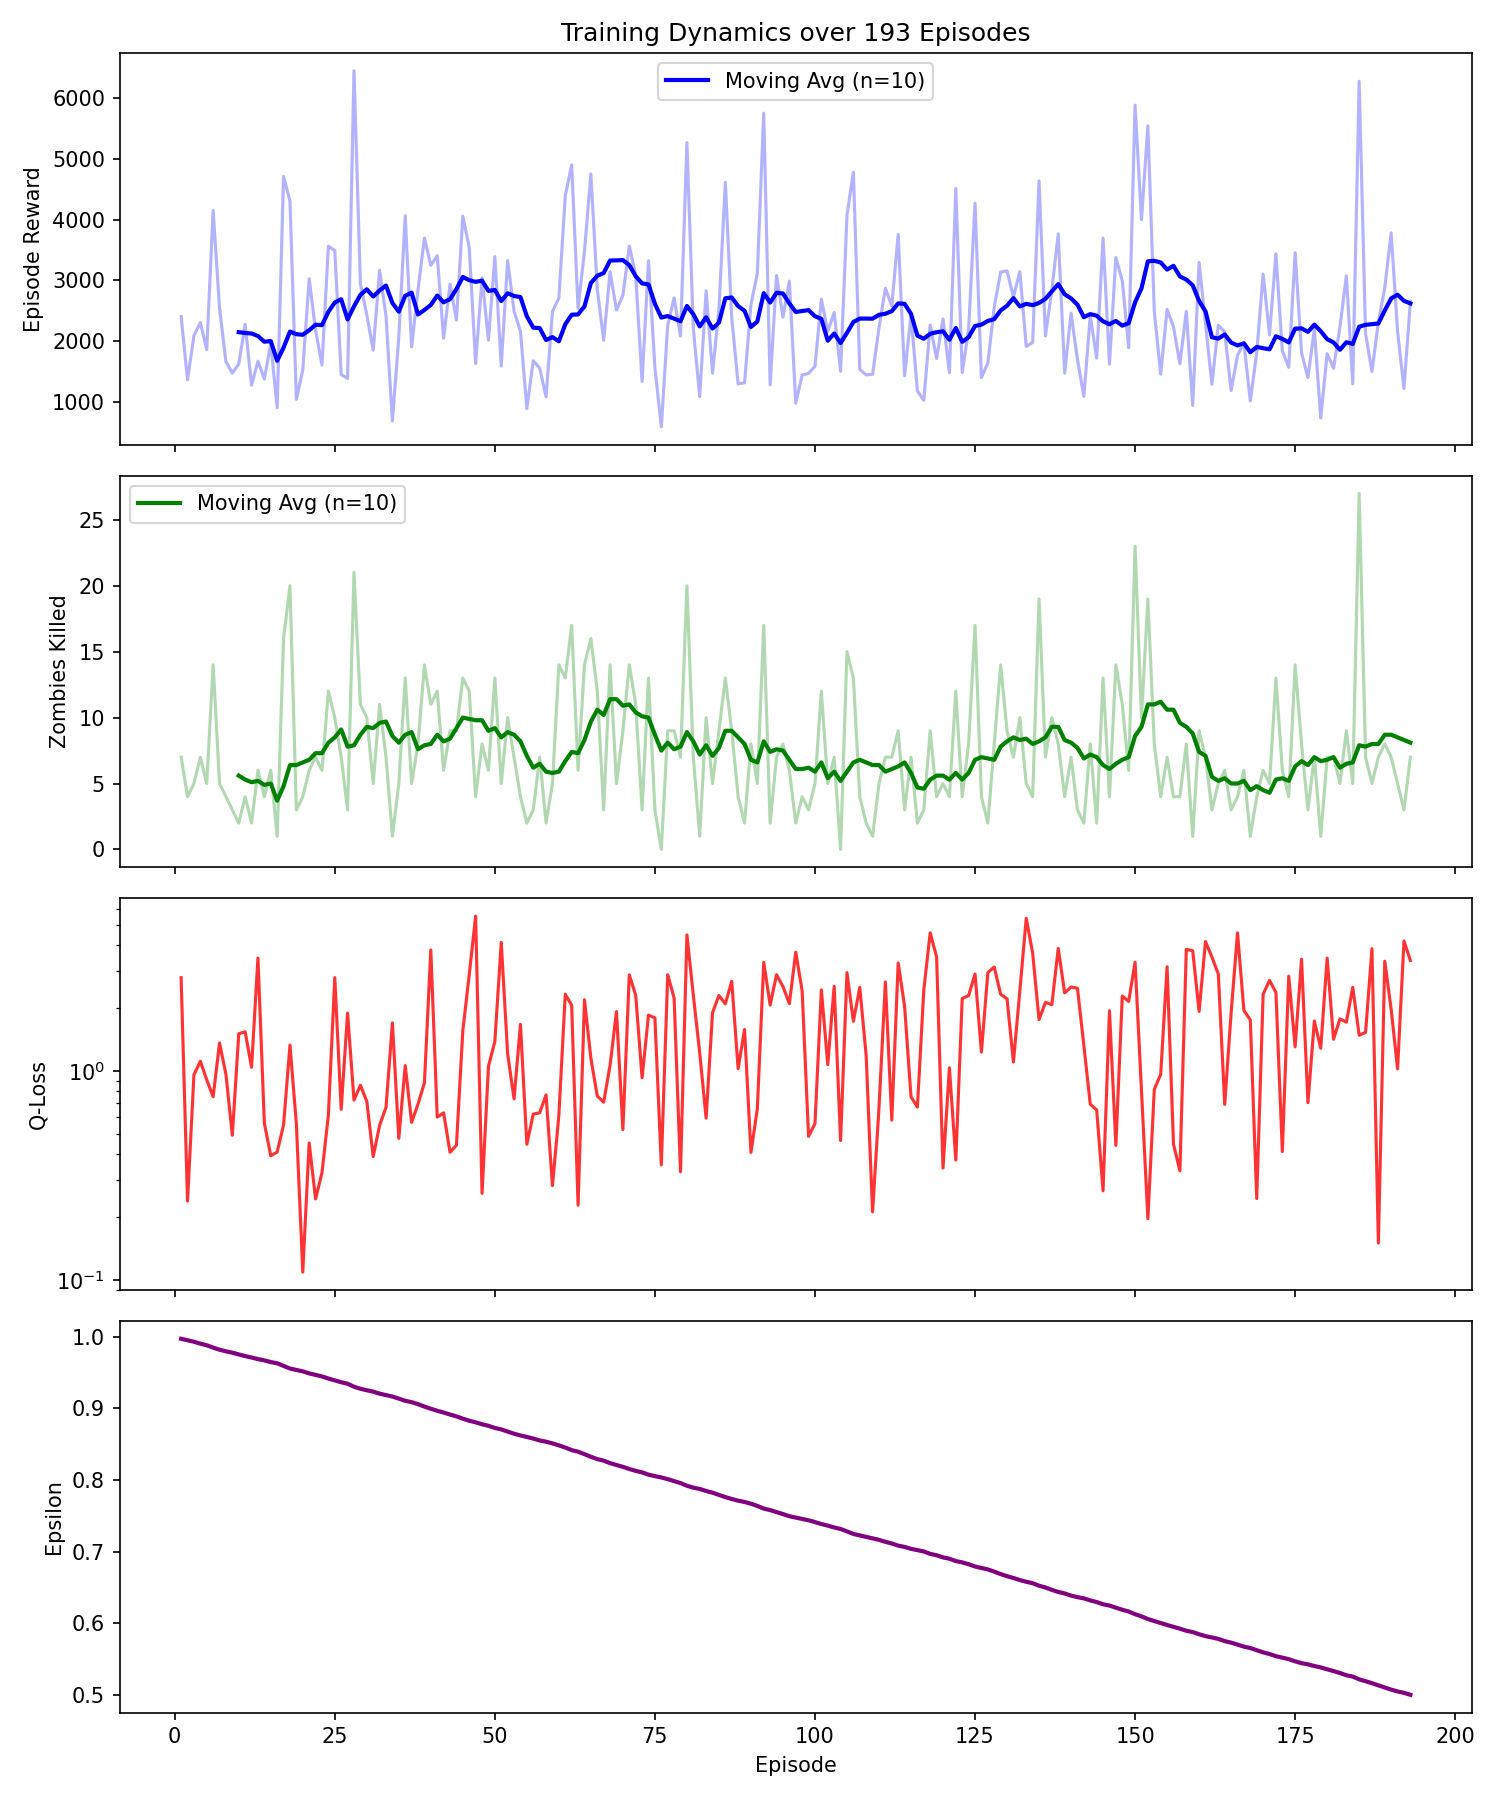
\includegraphics[width=\columnwidth]{training_curves.png}
\caption{Training dynamics over 193 episodes. (a) Episode reward with moving average shows a sustained trend. (b) Zombies killed per episode increases consistently. (c) Q-loss on log scale. (d) Epsilon decays linearly over training.}
\label{fig:curves}
\end{figure}

\begin{figure}[htbp]
\centering
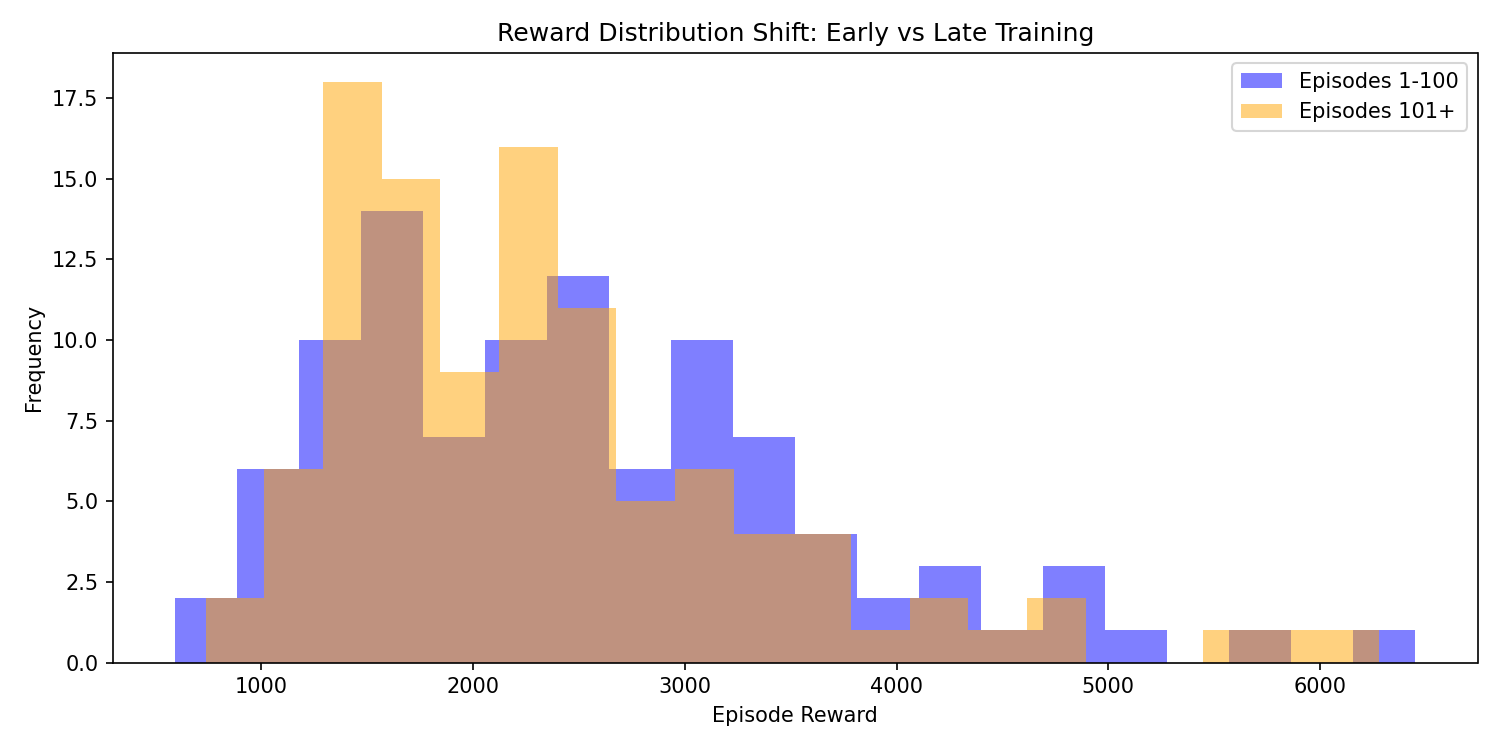
\includegraphics[width=\columnwidth]{reward_distribution.png}
\caption{Histogram of episode rewards. High variance reflects the stochastic nature of zombie spawn patterns and critical wave transitions.}
\label{fig:violin}
\end{figure}

\begin{figure}[htbp]
\centering
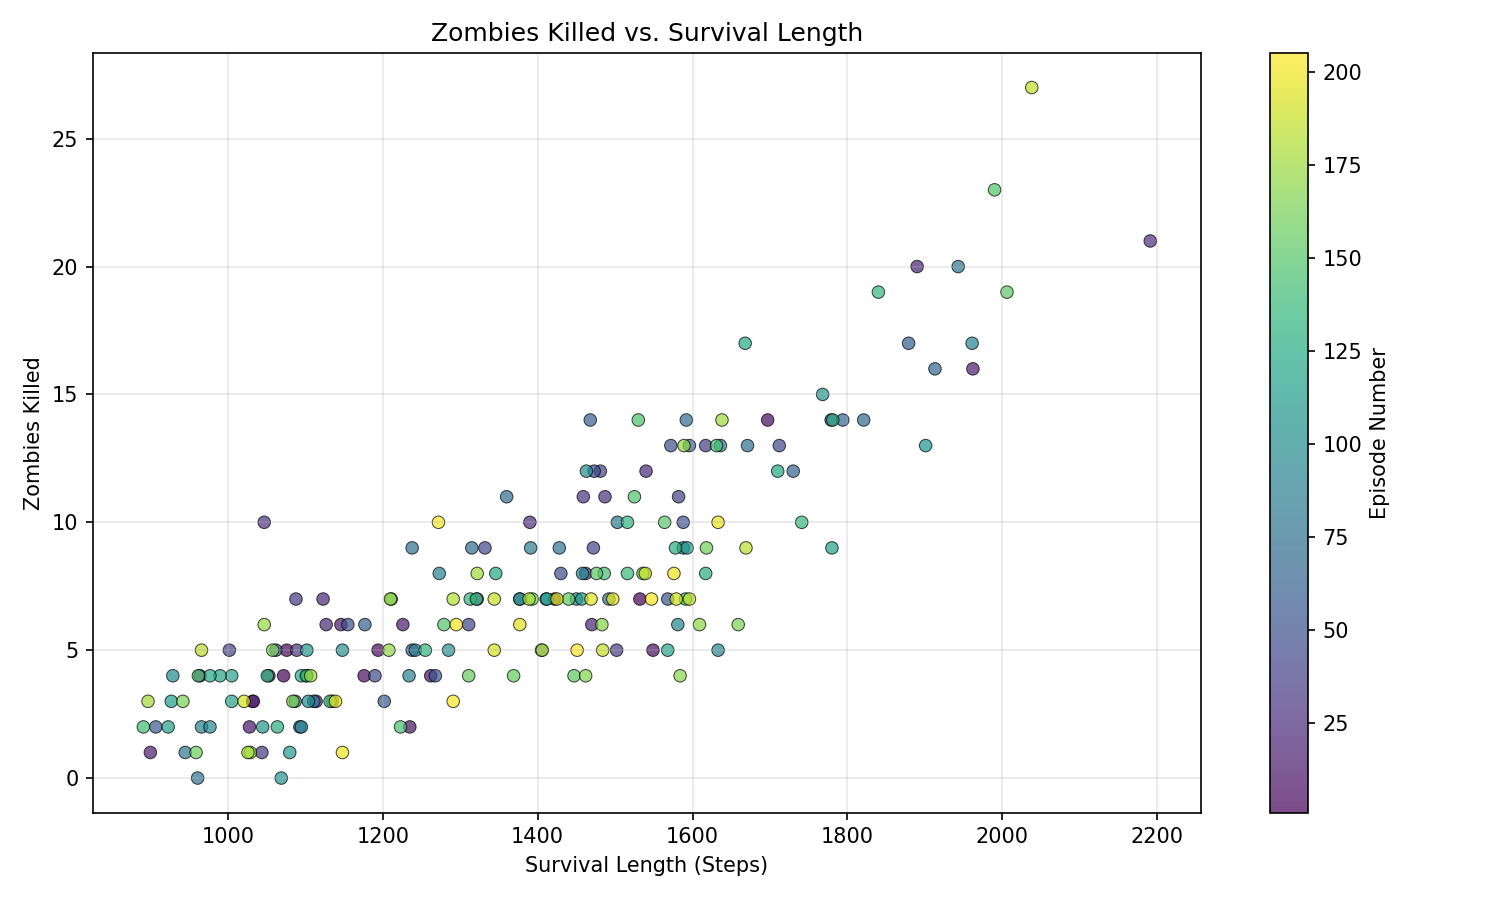
\includegraphics[width=\columnwidth]{kills_vs_length.png}
\caption{Zombies killed vs.\ episode survival length, colored by episode number. Later episodes (yellow) cluster towards higher survival times and higher kill counts.}
\label{fig:scatter}
\end{figure}

\subsection{Video and Simulation Demonstration}
A visual representation of the simulation provides essential debugging feedback, displaying the physical grid alongside real-time metrics including: current sun points, score, zombie kill count, current wave progress, game tick, and the number of alive zombies. Videos generated from the training checkpoints show the agent placing Peashooters and Repeaters in zombie-occupied lanes, successfully surviving multiple waves of Normal and Conehead zombies.

%===================================================================
\section{Problems Encountered and Solutions}
%===================================================================

This section documents the full chain of reward and environment engineering challenges---the central practical contribution of this paper.

\subsection{Problem 1: Reward Hacking --- ``Do Nothing'' Strategy}
\textbf{Symptom:} The first reward function penalized plant loss ($-50$ per plant destroyed). The agent discovered that placing \emph{no plants at all} was locally optimal: zero plants eaten $\to$ zero penalties. It preferred the $-200$ game-over penalty over $-250$ (game-over + one plant eaten).

\textbf{Root Cause:} Classic reward hacking. The penalty for plant loss exceeded the marginal benefit of surviving longer.

\textbf{Fix:} Added dense \emph{action-based} rewards: $+5.0$ per projectile hit and $+2.0$ per sun collected, making planting more valuable than inaction.

\subsection{Problem 2: Action Masking --- Exploration Collapse}
\textbf{Symptom:} Standard PPO without action masking. With 316 possible actions and only 2--5 valid per state, the agent's random exploration almost never sampled a valid action. The network learned to output uniform probability.

\textbf{Root Cause:} In a 316-action space with ${\sim}1\%$ valid actions, an unmasked agent needs ${\sim}316$ random steps to find one valid planting action.

\textbf{Fix:} Implemented custom action masking for the MCTS/DDQN pipeline to prune invalid branches. The agent immediately began exploring plant placements.

\subsection{Problem 3: Starting Sun Too Low}
\textbf{Symptom:} Default starting sun was 50. The agent spent it on a Wall-nut (cheapest option), depleted sun to 0, then had no resources for shooting plants. Videos showed 1--2 Wall-nuts with zero Peashooters.

\textbf{Fix:} Increased starting sun to 150. With 150 sun, the agent can immediately afford one Peashooter.

\subsection{Problem 4: Reward Always Negative --- No Positive Signal}
\textbf{Symptom:} The agent appeared not to be learning as episodic rewards remained deeply negative.

\textbf{Root Cause:} Game-over penalty was $-300$. Unless the agent killed enough zombies to earn $+300$ in rewards, net reward was always negative. The dominant terminal penalty masked genuine strategic progress.

\textbf{Fix:} Rebalanced reward scale: increased \texttt{projectile\_hit\_reward} from 0.005 to 5.0, added \texttt{sun\_reward}$=$2.0, set \texttt{plant\_damage\_penalty}$=$0.0 (Wall-nuts absorbing damage is correct behavior).

\subsection{Problem 5: Plants Not Shooting --- Wrong Plant Preference}
\textbf{Symptom:} After fixing starting sun, videos showed Wall-nuts and Potato Mines but no Peashooters. No projectiles visible.

\textbf{Root Cause:} Wall-nut costs 50 sun (affordable immediately), Peashooter costs 100. The Q-network learned Wall-nut placement was ``safe.''

\textbf{Fix:} Added \texttt{lane\_wasting\_penalty}$=$25.0---placing a non-shooter in a row with approaching zombies is penalized. This forced the agent to prefer Peashooters/Repeaters in contested lanes.

\subsection{Problem 6: MCTS Computational Cost on CPU}
\textbf{Symptom:} Full MCTS training with 50 simulations/step required up to 110 seconds per episode.

\textbf{Root Cause:} Each simulation requires a full \texttt{deep\_copy(PvZEngine)}. At 50 sims/step $\times$ 1,350 steps/episode = 67,500 copies per episode.

\textbf{Mitigation:} Implemented a dedicated \texttt{mcts\_replay\_buffer} so MCTS transitions are stored and reused by the DDQN without recalculating deep copies.

%===================================================================
\section{Discussion}
%===================================================================

\subsection{What Worked}
\begin{itemize}[leftmargin=*,nosep]
    \item \textbf{Wave Bonus reward} was highly effective: combining kill, projectile-hit, sun, and lane-wasting signals provided dense, consistent feedback.
    \item \textbf{Action masking} was critical. Without it, exploration in the 316-action space was statistically improbable.
    \item \textbf{MCTS lookahead} efficiently produced better action distributions than pure $\varepsilon$-greedy exploration, acting as a powerful teacher for the DDQN network.
\end{itemize}

\subsection{What Did Not Work As Expected}
\begin{itemize}[leftmargin=*,nosep]
    \item \textbf{Full Survival} across all 5 waves was rarely achieved. The final wave (15 zombies + Flag) often overwhelmed the defenses built during early waves, highlighting the extreme difficulty of resource management in the late game.
    \item \textbf{Potential-based shaping} was practically equivalent to Wave Bonus; the zombie-distance potential did not add useful learning signal beyond standard kill rewards.
    \item \textbf{Sparse reward} showed zero progress---the agent never received the ultimate reward to learn from, rendering learning impossible in early stages.
\end{itemize}

%===================================================================
\section{Conclusion}
%===================================================================

We presented a hybrid MCTS+DDQN reinforcement learning system for Plants vs.\ Zombies, marking the first time deep AlphaZero-style methods have been successfully deployed in this environment. The dominant challenge was \textbf{reward engineering}: multiple reward hacking and incentive misalignment failures were resolved through careful shaping design. Our DualNet and DuelingDDQN architecture proved capable of bidirectional learning, with MCTS providing lookahead planning and DDQN anchoring the value network. The final Wave Bonus reward scheme with action masking produced consistent, measurable learning, improving average kills by 44.6\% and survival length by 10.4\% over 193 episodes. The agent demonstrates genuine strategic behavior---placing shooters in zombie-occupied lanes, surviving multiple waves, and collecting sun for economic development. Future work will focus on extended CPU-parallel training, GPU-accelerated MCTS, and curriculum learning from low to high difficulty to achieve perfect survival rates.

%===================================================================
% REFERENCES
%===================================================================
\begin{thebibliography}{9}

\bibitem{silver2016}
D.~Silver et al., ``Mastering the game of Go with deep neural networks and tree search,'' \emph{Nature}, vol.~529, pp.~484--489, 2016.

\bibitem{silver2018}
D.~Silver et al., ``A general reinforcement learning algorithm that masters chess, shogi, and Go through self-play,'' \emph{Science}, vol.~362, no.~6419, pp.~1140--1144, 2018.

\bibitem{ng1999}
A.~Y.~Ng, D.~Harada, and S.~Russell, ``Policy invariance under reward transformations: Theory and application to reward shaping,'' in \emph{Proc. ICML}, 1999, pp.~278--287.

\bibitem{mnih2015}
V.~Mnih et al., ``Human-level control through deep reinforcement learning,'' \emph{Nature}, vol.~518, pp.~529--533, 2015.

\bibitem{schrittwieser2020}
J.~Schrittwieser et al., ``Mastering Atari, Go, chess and shogi by planning with a learned model,'' \emph{Nature}, vol.~588, pp.~604--609, 2020.

\bibitem{schulman2017}
J.~Schulman et al., ``Proximal policy optimization algorithms,'' \emph{arXiv:1707.06347}, 2017.

\bibitem{hasselt2016}
H.~van Hasselt, A.~Guez, and D.~Silver, ``Deep reinforcement learning with double Q-learning,'' in \emph{Proc. AAAI}, 2016, pp.~2094--2100.

\bibitem{schaul2016}
T.~Schaul et al., ``Prioritized experience replay,'' in \emph{Proc. ICLR}, 2016.

\bibitem{pvzrl}
ilovesodaa, ``pvz-rl: Plants vs.\ Zombies Reinforcement Learning Environment,'' GitHub, 2024. \url{https://github.com/ilovesodaa/pvz-rl}

\bibitem{clark2016}
J.~Clark and D.~Amodei, ``Faulty reward functions in the wild,'' OpenAI Blog, 2016.

\end{thebibliography}

\end{document}
